\documentclass[aspectratio=169]{beamer}

\usetheme{Madrid}
\usecolortheme{default}

\usepackage[utf8]{inputenc}
\usepackage[T1]{fontenc}
\usepackage[brazil]{babel}
\usepackage{graphicx}
\usepackage{hyperref}
\usepackage{xcolor}
\usepackage{booktabs}
\usepackage{listings}

\definecolor{oceanblue}{RGB}{0,74,119}
\definecolor{oceanlight}{RGB}{219,238,244}
\definecolor{oceangreen}{RGB}{0,120,110}

\setbeamercolor{structure}{fg=oceanblue}
\setbeamercolor{frametitle}{fg=white,bg=oceanblue}
\setbeamercolor{title}{fg=white,bg=oceanblue}
\setbeamercolor{block title}{fg=white,bg=oceangreen}
\setbeamercolor{block body}{bg=oceanlight}

\lstset{
  basicstyle=\ttfamily\small,
  breaklines=true,
  frame=single,
  backgroundcolor=\color{gray!8}
}

\IfFileExists{curso-beamer.sty}{\usepackage{curso-beamer}}{}

\newcommand{\figplaceholder}[1]{%
  \begin{center}
  \fbox{\begin{minipage}[c][4.5cm][c]{0.9\linewidth}
  \centering\small Figura esperada: \texttt{#1}
  \end{minipage}}
  \end{center}
}

\title[Introdução ao Curso]{Aula 0 --- Introdução ao Curso}
\subtitle{Arquiteturas Cloud-Native e Formatos Modernos de Dados para Oceanografia Operacional,\\
Clima e Meteorologia em Escala de Múltiplos Terabytes (Arq-Cloud)}
\author{Tobias Ferreira}
\institute{Instituto Nacional de Pesquisas Oceânicas (INPO)}
\date{01/09/2026}

\begin{document}

% ------------------------------------------------
\begin{frame}[plain,noframenumbering]
  \titlepage
\end{frame}

% ------------------------------------------------
\begin{frame}{Atividade inicial: que dados você usa?}
Antes de começarmos, vamos entender melhor a experiência do grupo.

\vspace{0.3cm}

No documento compartilhado \textbf{CodiMD}, escreva:

\begin{enumerate}
  \item uma frase sobre os dados com que você costuma trabalhar e o tamanho aproximado deles;
  \item um desafio que você já enfrentou com dados grandes demais ou lentos demais para processar;
  \item uma ferramenta, biblioteca ou sistema computacional que você já usou para análise, armazenamento ou acesso a dados.
\end{enumerate}

\vspace{0.3cm}

\begin{block}{Objetivo}
Conectar os conceitos do curso com problemas reais trazidos pelos participantes.
\end{block}
\end{frame}

% ------------------------------------------------
\begin{frame}{Jargon busting}
\Large
Antes de avançarmos, vamos alinhar alguns termos que aparecerão ao longo do curso.

\vspace{0.5cm}

\begin{block}{Por que isso importa?}
Muitos problemas com dados grandes aparecem porque usamos as mesmas palavras para coisas diferentes: memória, armazenamento, processo, thread, cluster, nuvem, bucket, formato, metadados.
\end{block}
\end{frame}

% ------------------------------------------------
\begin{frame}{CPU, core, processo e thread}
\begin{columns}
\column{0.48\textwidth}
\begin{itemize}
  \item \textbf{CPU}: unidade que executa instruções e cálculos.
  \item \textbf{Core}: uma unidade de processamento dentro da CPU.
  \item \textbf{Processo}: uma instância de um programa em execução.
  \item \textbf{Thread}: unidade menor de trabalho dentro de um processo.
\end{itemize}

\column{0.52\textwidth}
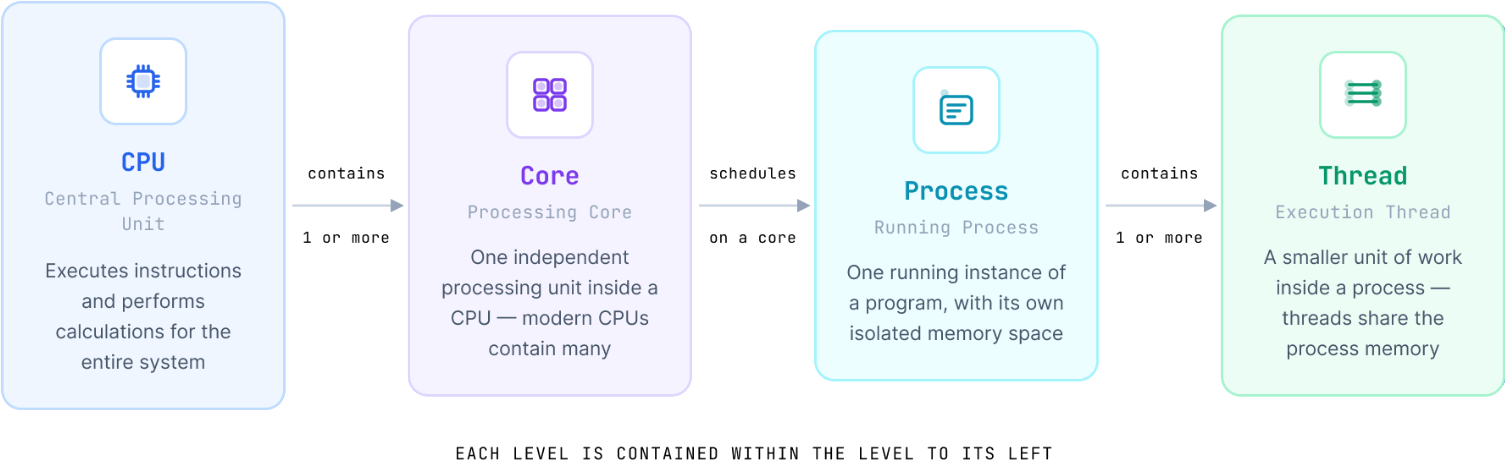
\includegraphics[width=\textwidth]{../episodes/fig/cpu_core_process_thread.png}
\end{columns}
\end{frame}

% ------------------------------------------------
\begin{frame}{Processamento paralelo e Dask}
\Large
Processamento paralelo significa dividir uma tarefa em partes menores que podem ser executadas ao mesmo tempo.

\vspace{0.4cm}

\begin{block}{Dask}
Dask é uma biblioteca Python que organiza grandes computações em tarefas menores, que podem ser executadas em paralelo em cores, processos ou workers.
\end{block}

\vspace{0.3cm}

\centering
\textbf{A ideia é trabalhar com dados maiores sem depender de uma única operação gigante.}
\end{frame}

% ------------------------------------------------
\begin{frame}{RAM e armazenamento}
\begin{columns}
\column{0.5\textwidth}
\begin{block}{RAM}
Memória de curto prazo do computador. É rápida, mas limitada.
\end{block}

\begin{itemize}
  \item usada durante cálculos;
  \item pode limitar análises grandes;
  \item desaparece quando o processo termina.
\end{itemize}

\column{0.5\textwidth}
\begin{block}{Armazenamento}
Onde os dados vivem de forma mais permanente.
\end{block}

\begin{itemize}
  \item disco local ou SSD;
  \item storage compartilhado;
  \item object storage;
  \item sistemas de arquivos em HPC.
\end{itemize}
\end{columns}
\end{frame}

% ------------------------------------------------
\begin{frame}{Cluster, node e HPC}
\begin{columns}
\column{0.46\textwidth}
\begin{itemize}
  \item \textbf{Cluster}: conjunto de computadores conectados.
  \item \textbf{Node}: um computador dentro do cluster.
  \item \textbf{HPC}: sistema compartilhado para computação pesada e processamento de grandes volumes de dados.
\end{itemize}

\vspace{0.2cm}

\begin{block}{Exemplo}
O JASMIN é uma infraestrutura usada para ciência ambiental intensiva em dados.
\end{block}

\column{0.54\textwidth}
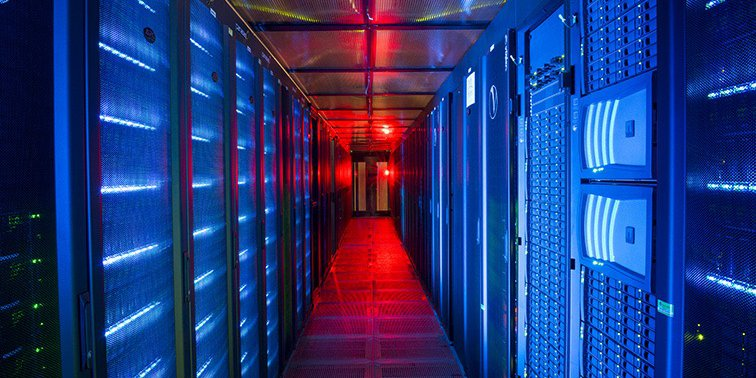
\includegraphics[height=5.5cm]{../episodes/fig/hpc.png}
{\tiny Fonte: JASMIN.}
\end{columns}
\end{frame}

% ------------------------------------------------
\begin{frame}{JASMIN e SSH}
\begin{columns}
\column{0.47\textwidth}
\textbf{JASMIN} é a infraestrutura do Reino Unido para análise de dados ambientais intensivos.

\vspace{0.3cm}

Ela oferece:
\begin{itemize}
  \item notebooks;
  \item armazenamento compartilhado;
  \item recursos computacionais;
  \item ambientes para dados grandes.
\end{itemize}

\vspace{0.2cm}

\textbf{SSH} é uma forma segura de conectar a computadores remotos.

\column{0.53\textwidth}
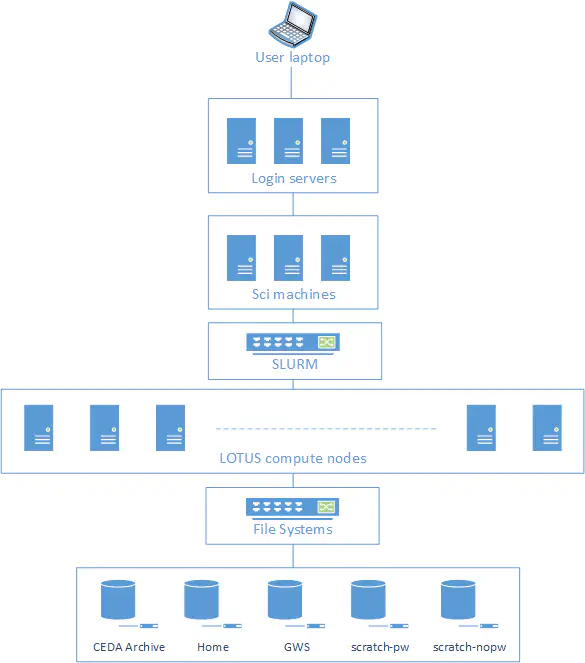
\includegraphics[height=6.5cm]{../episodes/fig/jasmin.png}
\end{columns}
\end{frame}

% ------------------------------------------------
\begin{frame}{Group workspace}
\Large
Um \textbf{group workspace} é uma área de armazenamento compartilhada no JASMIN.

\vspace{0.4cm}

\begin{itemize}
  \item permite colaboração entre usuários;
  \item evita múltiplas cópias locais dos mesmos dados;
  \item facilita o acesso aos dados do curso;
  \item aproxima o processamento do local onde os dados estão armazenados.
\end{itemize}
\end{frame}

% ------------------------------------------------
\begin{frame}{Jupyter notebook e kernel}
\begin{columns}
\column{0.5\textwidth}
\begin{block}{Jupyter notebook}
Ambiente no navegador para combinar código, texto, resultados, tabelas e gráficos.
\end{block}

\begin{itemize}
  \item útil para exploração;
  \item facilita demonstrações;
  \item permite documentação junto com o código.
\end{itemize}

\column{0.5\textwidth}
\begin{block}{Kernel}
Ambiente Python que executa o código do notebook.
\end{block}

\begin{itemize}
  \item define quais pacotes estão disponíveis;
  \item mantém variáveis em memória;
  \item pode ser reiniciado durante o trabalho.
\end{itemize}
\end{columns}
\end{frame}

% ------------------------------------------------
\begin{frame}[fragile]{\texttt{environment.yml}, conda e mamba}
\texttt{environment.yml} descreve a versão do Python e os pacotes necessários para reproduzir o ambiente.

\vspace{0.3cm}

\begin{lstlisting}[language=bash]
conda env create -f environment.yml
conda activate cloud-native-geoscience-course
\end{lstlisting}

\vspace{0.3cm}

\begin{itemize}
  \item \textbf{conda}: gerencia ambientes e pacotes.
  \item \textbf{mamba}: alternativa mais rápida para resolver e instalar pacotes.
\end{itemize}
\end{frame}

% ------------------------------------------------
\begin{frame}{Dataset, array, coordenada e variável}
\begin{columns}
\column{0.5\textwidth}
\begin{itemize}
  \item \textbf{Dataset}: conjunto de dados e metadados relacionados.
  \item \textbf{Array}: grade multidimensional de valores.
  \item \textbf{Coordenada}: eixo nomeado, como tempo, latitude, longitude ou profundidade.
  \item \textbf{Variável}: valor medido ou modelado, como temperatura ou salinidade.
\end{itemize}

\column{0.5\textwidth}
\Large
\[
T = T(x, y, z, t)
\]

\vspace{0.3cm}

\begin{block}{Exemplo}
Temperatura do oceano variando no espaço, na profundidade e no tempo.
\end{block}
\end{columns}
\end{frame}

% ------------------------------------------------
\begin{frame}{Metadados e vocabulário controlado}
\Large
\textbf{Metadados} são informações que explicam o que os dados significam.

\vspace{0.3cm}

\begin{itemize}
  \item unidades;
  \item nomes longos;
  \item coordenadas;
  \item dimensões;
  \item projeções;
  \item convenções e atributos.
\end{itemize}

\vspace{0.3cm}

\begin{block}{Vocabulário controlado}
Lista padronizada de termos e identificadores para reduzir ambiguidade.
\end{block}
\end{frame}

% ------------------------------------------------
\begin{frame}{Zarr, Xarray, chunk e lazy loading}
\begin{itemize}
  \item \textbf{Zarr}: formato chunked para arrays N-dimensionais grandes.
  \item \textbf{Xarray}: biblioteca Python para trabalhar com arrays rotulados e metadados.
  \item \textbf{Chunk}: pedaço menor de um array grande.
  \item \textbf{Lazy loading}: os dados não são lidos completamente ao abrir o dataset; são carregados apenas quando necessário.
\end{itemize}

\vspace{0.4cm}

\begin{block}{Ideia prática}
Abrir um dataset grande não significa colocar todo o dataset na memória.
\end{block}
\end{frame}

% ------------------------------------------------
\begin{frame}{Object storage e bucket}
\begin{columns}
\column{0.46\textwidth}
Object storage guarda dados como objetos independentes, geralmente acessados por APIs como S3.

\vspace{0.3cm}

\begin{itemize}
  \item \textbf{Bucket}: contêiner principal para objetos.
  \item \textbf{Object}: unidade armazenada, com dados e metadados.
  \item Muito usado em nuvem e em fluxos cloud-native.
\end{itemize}

\column{0.54\textwidth}
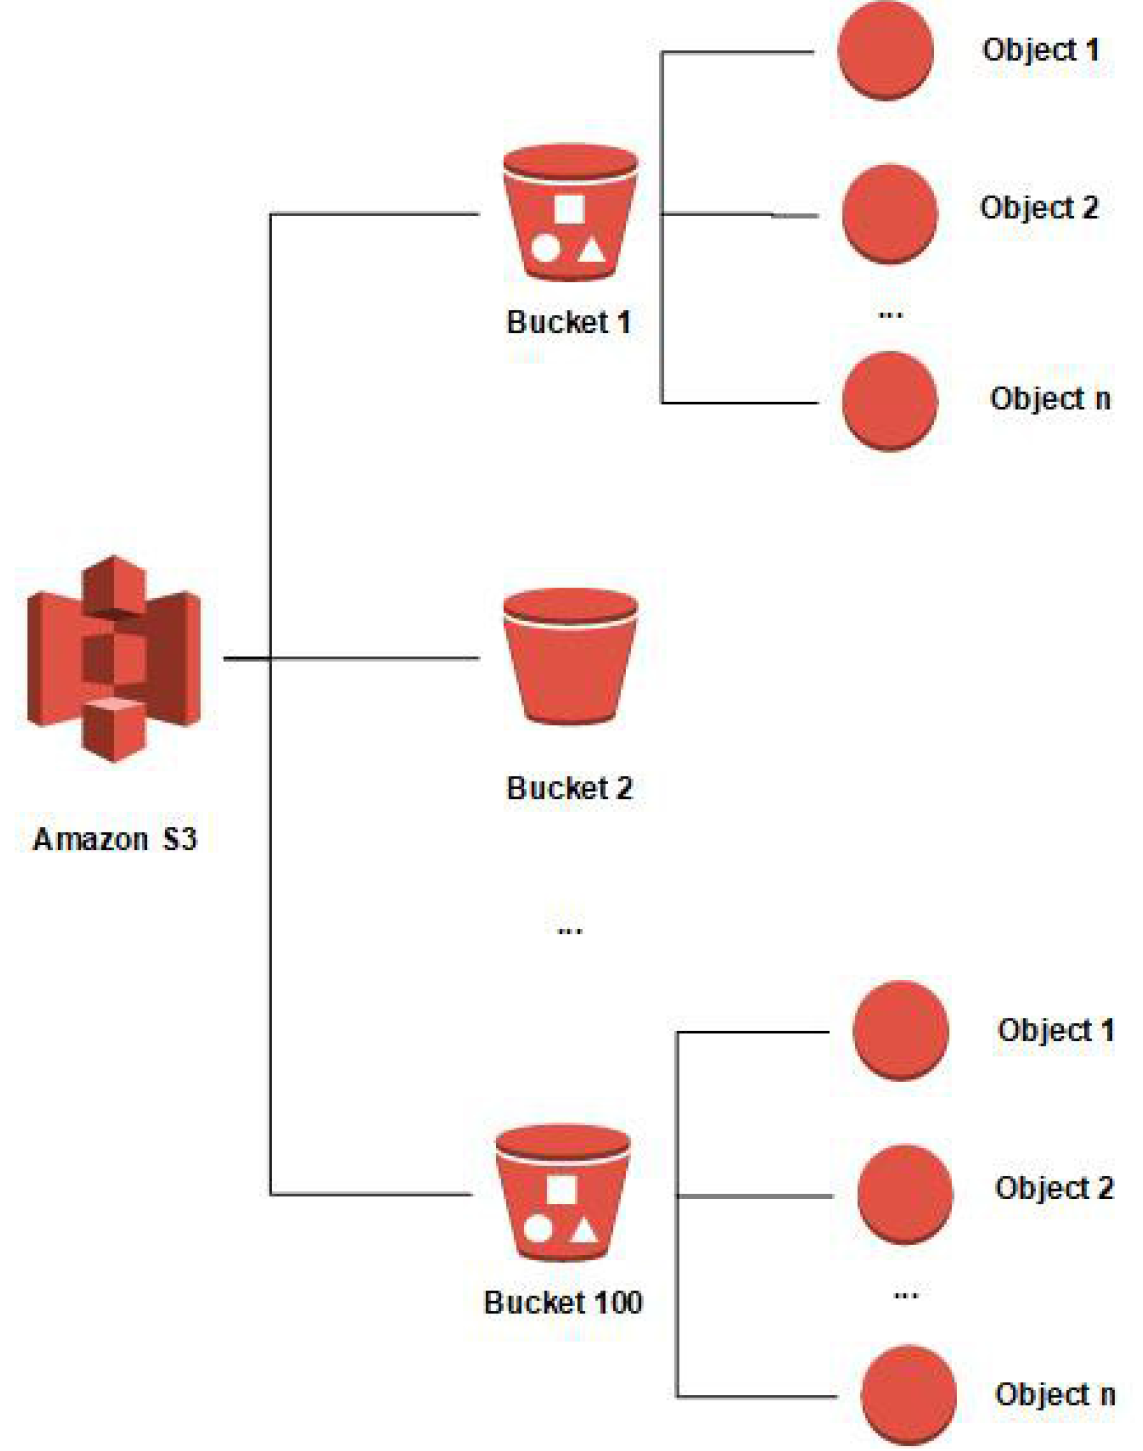
\includegraphics[width=\textwidth]{../episodes/fig/bucket_and_object_store.png}
{\tiny Fonte: IT Konekt.}
\end{columns}
\end{frame}

% ------------------------------------------------
\begin{frame}{POSIX versus object store}
\begin{columns}
\column{0.5\textwidth}
\textbf{Sistema POSIX}
\begin{itemize}
  \item arquivos e diretórios;
  \item caminhos tradicionais;
  \item disco local ou filesystem compartilhado;
  \item muito comum em HPC.
\end{itemize}

\column{0.5\textwidth}
\textbf{Object store}
\begin{itemize}
  \item objetos acessados por API;
  \item buckets e chaves;
  \item bom para acesso remoto e paralelo;
  \item não se comporta exatamente como um disco tradicional.
\end{itemize}
\end{columns}

\vspace{0.4cm}

\begin{block}{Consequência}
Nem todo fluxo pensado para arquivos locais funciona bem em object storage.
\end{block}
\end{frame}

% ------------------------------------------------
\begin{frame}{Formato cloud-native}
\Large
Um formato \textbf{cloud-native} é desenhado para funcionar bem com acesso remoto e object storage.

\vspace{0.4cm}

Normalmente ele permite:

\begin{itemize}
  \item leitura parcial dos dados;
  \item acesso paralelo;
  \item redução de downloads completos;
  \item melhor integração com processamento distribuído;
  \item compartilhamento mais eficiente.
\end{itemize}
\end{frame}

% ------------------------------------------------
\begin{frame}{STAC}
\begin{columns}
\column{0.45\textwidth}
\textbf{STAC} é um padrão para descrever e organizar assets geoespaciais.

\vspace{0.3cm}

\begin{itemize}
  \item facilita descoberta de dados;
  \item organiza coleções, itens e assets;
  \item conecta metadados com arquivos e serviços;
  \item é muito usado em catálogos cloud-native.
\end{itemize}

\column{0.55\textwidth}
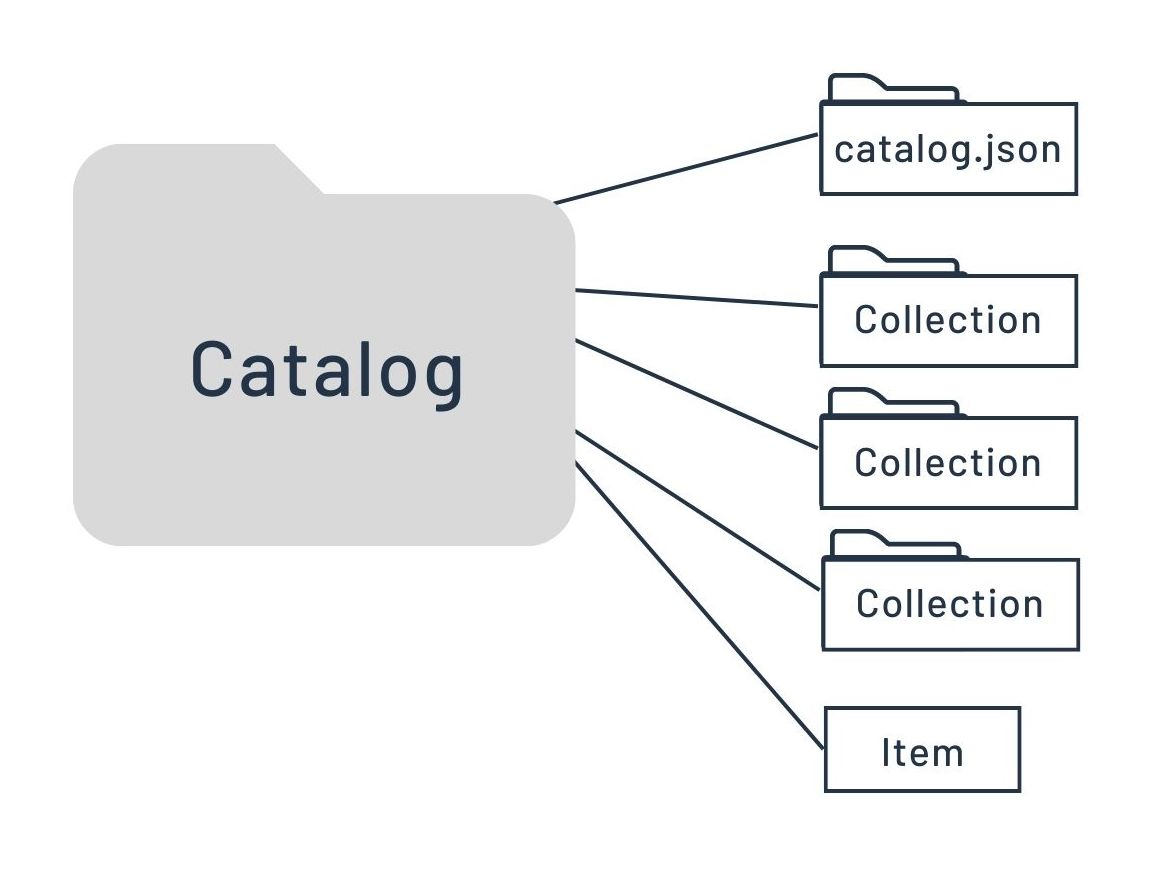
\includegraphics[width=\textwidth]{../episodes/fig/stac_example.png}
{\tiny Fonte: STAC.}
\end{columns}
\end{frame}

% ------------------------------------------------
\begin{frame}{Icechunk e VirtualiZarr}
\begin{columns}
\column{0.5\textwidth}
\begin{block}{Icechunk}
Adiciona versionamento, histórico e controle de mudanças a stores Zarr.
\end{block}

\begin{itemize}
  \item branches;
  \item tags;
  \item reprodutibilidade;
  \item rastreamento de alterações.
\end{itemize}

\column{0.5\textwidth}
\begin{block}{VirtualiZarr}
Permite trabalhar com arquivos existentes como se fossem datasets Zarr, sem copiar todos os dados.
\end{block}

\begin{itemize}
  \item útil para migração gradual;
  \item reduz cópias;
  \item cria uma camada virtual de acesso.
\end{itemize}
\end{columns}
\end{frame}

% ------------------------------------------------
\begin{frame}{Multiscale e pirâmide}
\Large
Um dataset \textbf{multiscale} armazena a mesma informação em múltiplas resoluções.

\vspace{0.4cm}

Uma \textbf{pirâmide} é a estrutura em camadas que permite visualizar rapidamente uma versão mais grosseira e depois aproximar para níveis mais detalhados.

\vspace{0.4cm}

\begin{block}{Por que isso importa?}
É uma estratégia essencial para visualização eficiente de grandes datasets na web.
\end{block}
\end{frame}

% ------------------------------------------------
\begin{frame}{Como esses conceitos aparecem no curso}
\begin{itemize}
  \item Começamos com os desafios de dados N-dimensionais e formatos tradicionais.
  \item Depois discutimos object storage, acesso parcial e formatos cloud-native.
  \item Em seguida, usamos Zarr, Dask e ferramentas de conversão.
  \item Também veremos catálogos STAC, versionamento com Icechunk e visualização web.
\end{itemize}

\vspace{0.4cm}

\begin{block}{Relação com o curso}
Mover menos dados, processar de forma mais inteligente e tornar o fluxo mais reproduzível.
\end{block}
\end{frame}

% ------------------------------------------------
\begin{frame}{Resumo}
\begin{itemize}
  \item O curso apresenta fluxos cloud-native para dados ambientais grandes.
  \item O foco está em oceanografia, clima e meteorologia.
  \item Vamos trabalhar com formatos, processamento paralelo, object storage, catálogos e visualização.
  \item Conceitos como CPU, RAM, cluster, chunk, lazy loading e metadados serão usados durante todo o curso.
\end{itemize}
\end{frame}

\end{document}
